\documentclass{beamer}

% \usepackage{beamerthemesplit} // Activate for custom appearance

%\setbeamertemplate{navigationsymbols}{}
\usenavigationsymbolstemplate{}
\usepackage{amsmath, amssymb, setspace, amsthm, stackrel}
\usepackage{arydshln}

% graphics stuff
\usepackage{graphicx}
\usepackage{caption}
\usepackage{subcaption}
\captionsetup{compatibility=false}
%\usepackage{tabularx}

% Bibtex related stuff
\usepackage{natbib}
\bibpunct{(}{)}{;}{a}{}{,}


\newtheorem{thm}{Theorem}
%%%%%%%%%%%%%%%%%%%%%%%%%%%%%%%%%%%%%%%%%%%%%
% list of user-defined commands
%%%%%%%%%%%%%%%%%%%%%%%%%%%%%%%%%%%%%%%%%%%%
\renewcommand{\L}{\mathcal{L}}
\renewcommand{\S}{\mathcal{S}}
\renewcommand{\P}{\mathcal{P}}
\newcommand{\A}{\mathcal{A}}
\newcommand{\C}{\mathcal{C}}
\newcommand{\X}{\mathcal{X}}
\newcommand{\Y}{\mathcal{Y}}
\newcommand{\T}{\mathcal{T}}
\newcommand{\N}{\mathcal{N}}
\newcommand{\Tmat}{\mathbf{T}}
\newcommand{\Rmat}{\mathbf{R}}
%\renewcommand{\H}{\ensuremath{\mathcal{H}}}
\newcommand{\R}[1]{\ensuremath{ R_{#1} }}
%\newcommand{\RR}[2]{\ensuremath{ R_{#1<#2>} }}
\renewcommand{\H}{\mathcal{H}}
%\newcommand{\HH}[2]{\ensuremath{ R_{#1<#2>} }}
\newcommand{\tsum}{\ensuremath{\oplus}}
\newcommand{\tprod}{\ensuremath{\otimes}}
\newcommand{\tminus}{\ensuremath{\ominus}}
\newcommand{\Real}{\ensuremath{ \mathbb{R} }}
\newcommand{\norm}[1]{\left\|#1\right\|}
\newcommand{\bbeta}{\boldsymbol\beta}
\newcommand{\balpha}{\boldsymbol\alpha}
\newcommand{\bgamma}{\boldsymbol\gamma}
\newcommand{\bepsilon}{\boldsymbol\epsilon}
\newcommand{\blambda}{\boldsymbol\lambda}
\newcommand{\wh}[1]{\widehat{#1}}
\newcommand{\inner}[2]{\langle #1, #2 \rangle}

\newcommand{\hk}{H(R)}
\newcommand{\hkk}{H(R\otimes R)}



\title{Functional Data Analysis Approach to Land Cover Classification in India Using MERIS Terrestrial Chlorophyll Index Data}
		
\author{Daniel Fortin \\[0.5cm]
Iowa State University}	
		
\date{November 18, 2014}

\begin{document}

\frame{\titlepage}

%%%%% INTRODUCTION %%%%%

\begin{frame}[t]{Functional Data Analysis (FDA)}
	All data are discrete, so why adopt an FDA approach to analysis?
	
	\begin{quote}
 A functional data analysis approach is attractive when a primary variable of interest is best conceptualized as realizations of random smooth curves whose features require flexible estimation.
	\end{quote}
	\begin{itemize}
		\item observations are at such a high frequency that it makes practical sense to treat it as a continous variable
		\item Scientific questions of interest relate to properties of curves (e.g. derivatives)
		\item Estimation or prediction of the whole process is desired over a scalar summary of the curve
	\end{itemize}
\end{frame}
%--- Next Frame ---%
\begin{frame}[t]{Example: Human Growth Curves}
	\begin{figure}
	\begin{center}
	\includegraphics[width=0.8\textwidth]{Plots/growth-curves.png}
	\caption{ The heights of 10 girls measured at 31 ages.}
	\end{center}
	\end{figure}
\end{frame}
%--- Next Frame ---%

\begin{frame}[t]{Example: Temperature Profiles at Canadian Weather Stations}
	\begin{figure}
	\begin{center}
	\includegraphics[width=3in]{Plots/canadian-weather.pdf}
	\caption{ Mean monthly temperatures for Canadian weather stations.}
	\end{center}
	\end{figure}
\end{frame}

%--- Next Frame ---%

\frame{
\begin{figure}
        \centering
        \begin{subfigure}[b]{0.44\textwidth}
                \centering
                \includegraphics[width=\textwidth]{Plots/fourier-basis-7.pdf}
                \caption{Fourier basis functions}
        \end{subfigure}
         \begin{subfigure}[b]{0.44\textwidth}
                \centering
                \includegraphics[width=\textwidth]{Plots/bspline-basis-7-order4.pdf}
                \caption{B-spline basis functions}
        \end{subfigure}
 \end{figure}
}

\begin{frame}[t]{}
	\begin{tabular}{c|c|c|}
		& Independent & Dependent \\
		\hline
		Sparse & \includegraphics[width=1.3in]{Plots/canadian-weather.pdf} & \includegraphics[width=1.3in]{Plots/canadian-weather.pdf} \\
		\hline
		Dense & \includegraphics[width=1.3in]{Plots/growth-curves.png} &\includegraphics[width=1.3in]{Plots/canadian-weather.pdf}\\
		\hline
	\end{tabular}
\end{frame}
%--- Next Frame ---%



\frame{
Goals:
\begin{itemize}
\item Represent curves as linear combination of leading FPCs as empirical basis
\item Perform classification by utilizing multivariate techniques on basis coefficients
\end{itemize}
Outline:
\begin{enumerate}
\item Nonparametric covariance estimation and principal component function estimation
\item Application to phenology data
\end{enumerate}
}




%%%%% NONPARAMETRIC COVARIANCE FUNCTION ESTIMATION AND EIGENFUNCTION ESTIMATION %%%%%
\frame{
\begin{center}
NONPARAMETRIC COVARIANCE FUNCTION AND PRINCIPAL COMPONENT FUNCTION ESTIMATION FOR FUNCTIONAL DATA
\end{center}
}

\begin{frame}
\frametitle{Smoothing Penalty Approach (univariate case)}
\begin{equation*}
\widehat{f}_{\lambda} = \hspace{.07in}\stackrel[f \in \H]{}{\mbox{arg min}} \left\{ \frac{1}{n}\sum_{i=1}^{n}(y_i - f(x_i))^2 + \lambda\times Pen(f) \right\}.
\label{eq:PLS_norm}
\end{equation*}
\begin{itemize}
\item $Pen(f)$ is a penalty applied to 'non-smooth' functions in order to avoid over fitting the data.
\item $\H$ is an 'appropriate' function space.
\item $\lambda$ is a parameter which governed the trade-off between fitting the data and smoothness of the curve.
\end{itemize}
A reasonable approach is to define $Pen(f) = \int_0^1 (f'')^2dx$. 
\begin{equation*}
\widehat{f}_{\lambda} = \hspace{.07in}\stackrel[f \in \H]{}{\mbox{argmin}} \left\{ \frac{1}{n}\sum_{i=1}^{n}(y_i - f(t_i))^2 + \lambda\ \int_0^1(f'')^2dx \right\}
\label{eq:unpenalized objective function}
\end{equation*}
Okay, so how do we solve for $\hat{f}$?
\end{frame}

%%%%%%%%%%%%%%%%%%
%%%%%%%%%%%%%%%%%
\begin{frame}\frametitle{Spaces generated by positive definite functions}
\begin{itemize}
\item Let $K(x,y)$ be a symmetric positive-definite kernel function. 
\item $\H_K = \{K(\cdot, y), y \in \Real\}$
\end{itemize}
From Mercer's theorem $K(x,y)$ has the representation
\[K(x,y)=\sum_{i=0}^{\infty}\lambda_{i}\phi_{i}(x)\phi_{i}(y)\]
\begin{itemize}
\item $\phi_{i}$ are eigenfunctions of the kernel function $K$
corresponding to eigenvalues $\lambda_{i}$.
\item $\phi_{i}$ are basis for $L_2$.
\end{itemize}
$\H_{K}\subset L_{2}$ contains functions satisfying
\[f(x)=\sum_{i=1}^{\infty}c_{i}\phi_{i}(x)\] 
 for $c_{i} \mbox{ with  }\norm{f}_{\H_K}:= \sum_{i=1}^{\infty}\frac{{c_{i}^{2}}}{\lambda_{i}}<\infty$
\end{frame}

% \begin{frame}
% The minimization problem becomes
% \begin{equation*}
% \widehat{f}_{\lambda} = \hspace{.07in}\stackrel[\{c_j\}_{j=1}^{\infty}]{}{\mbox{argmin}} \left\{ \frac{1}{n}\sum_{i=1}^{n}(y_i - \sum_{j=1}^{\infty}c_j\phi_j(x_i))^2 + \lambda\ \sum_{j=1}^{\infty}\frac{c_j^2}{\lambda_j} \right\}
% \label{eq:unpenalized objective function}
% \end{equation*}
% The solution is finite dimensional and has the form
% \[
% \hat{f}(x)=\sum_{i=1}^{N}b_{i}K(x,x_{i})
% \]
% This remarkable result is due to the fact that $K(x,y)$ is a 'reproducing' kernel.
%
% That is great! And it gets better...
% \end{frame}
\begin{frame}
The reproducing property: 
\begin{itemize}
\item $f(x_i) = \inner{K(\cdot, x_i)}{f}$
\item $\inner{K(\cdot, x_i)}{K(\cdot, x_j)} = K(x_i, x_j)$
\end{itemize}
implies that for $f(x)=\sum_{i=1}^{N}b_{i}K(x,x_{i})$

\[\left\Vert f\right\Vert _{H_{K}}^{2}=\inner{f}{f}_{H_{K}}=\sum_{i=1}^{N}\sum_{j=1}^{N}b_{i}b_{j}K(x_{i},x_{j})\]

Thus the optimization reduces to minimizing, over choices of vectors $b$, the
following

\[(Y-Kb)'(Y-Kb)+\lambda b'Kb.\]
\end{frame}

\begin{frame}
\frametitle{Side Note: Some (very) useful Hilbert space properties:}

\begin{itemize}
\item tensor sum decomposition: \structure{$\H = \H_0 \tsum \H_1$}
	\begin{itemize}
	\item $f \in \H$ has representation $f = f_0 + f_1$
	\item If $\H_0$, $\H_1$ are RKHS, then \structure{$R = R_0 + R_1$} is r.k. on $\H$.
	\end{itemize}
	\vspace{1cm}
\item tensor product space: If $\H_{<1>}$ and $\H_{<2>}$ are RKHS then
\begin{itemize}
	\item Tensor product space \structure{$\H_{<1>}\tprod \H_{<2>}$} is a RKHS 
	\item $R_{<1>}\tprod R_{<2>}((s_1, t_1), (s_2, t_2)) = \structure{R_{<1>}(s_1, s_2)R_{<2>}(t_1, t_2)}$
	\end{itemize}
\end{itemize}
\end{frame}

\frame{
\frametitle{Back to the original problem...}

 Penelty based on high-order derivative
\begin{equation*}
\widehat{f}_{\lambda} = \hspace{.07in}\stackrel[f \in \H]{}{\mbox{argmin}} \left\{ \frac{1}{n}\sum_{i=1}^{n}(y_i - f(x_i))^2 + \lambda\ \int_0^1(f'')^2dx \right\}
\label{eq:unpenalized objective function}
\end{equation*}

Consider the space $\H =  \{f : f, f' \mbox{ absolutely continuous}, f'' \in L_2[0,1]\}$ with decomposition $\H = \H_0 \tsum \H_1$, where 
  \begin{align*}
  \H_0 &= \left\{f: \int_0^1(f'')^2dx = 0\right\}\\
  \H_1 & = \H \tminus \H_0
  \end{align*}
  The space $\H$ is a RKHS under the inner product
  \begin{align*}
  \inner{f}{g} &= \inner{f}{g}_0 + \inner{f}{g}_1 \\
  			&= \left(\int_0^1fdx\right)\left(\int_0^1gdx\right) + \left(\int_0^1f'dx\right)\left(\int_0^1g'dx\right) + \int_0^1 f''g''dx
  \end{align*}
}
\begin{frame}
\frametitle{}
  The minimization problem becomes
  \begin{equation*}
\widehat{f}_{\lambda} = \hspace{.07in}\stackrel[f \in \H]{}{\mbox{arg min}} \left\{ \frac{1}{n}\sum_{i=1}^{n}(y_i - f(x_i))^2 + \lambda\norm{P_1(f)}^2_{\H_1} \right\}.
\end{equation*}
where $P_1(f)=f_1$ is the projection of $f$ onto the space $\H_1$. \\[1cm]
The solution has the form
\begin{equation*}
	\hat{f}(t) = \sum_{j=1}^M d_j\phi_j(t) + \sum_{i=1}^N c_iR_1(x, x_i), 
	\label{eq:unpenalized solution}
\end{equation*}
\end{frame}

% \begin{frame}
%
% \begin{table}
% \begin{tabular}{|c|c|}
% \hline
% & Starting from kernel \\[0.3cm]
% \hline
% $[0,1]$ &$\hat{f}(t) =  \sum_{i=1}^N c_iR(t, t_i)$ \\[0.3cm]
% \hline
% $[0,1]\times [0,1]$ & Cai and Yuan (2010) \\[0.3cm]
% \hline
% \end{tabular}
% \end{table}
%
% \begin{table}
% \begin{tabular}{|c|c|}
% \hline
%  & Starting from penalty \\[0.3cm]
% \hline
% $[0,1]$ & $\hat{f}(t) = \sum_{j=1}^M d_j\phi_j(t) + \sum_{i=1}^N c_iR_1(t, t_i)$\\[0.3cm]
% \hline
% $[0,1]\times [0,1]$  & $?$\\[0.3cm]
% \hline
% \end{tabular}
% \end{table}
%
% The focus of our work is to fill in the remaining box, and to derive eigenfunctions for this estimator.
% \end{frame}

\begin{frame}\frametitle{Cai and Yuan (2010)}
Assume the sample path of $X$ belongs to an RKHS $H_{R}.$ Then we
can write

\[
X(\cdot)=\sum_{k\geq1}x_{k}\phi_{k}(\cdot)\]


where $x_{k}=(X,\phi_{k})_{L_{2}}$.

The covariance function $C_{0}(s,t)$ is given by

\[
C_{0}(s,t)=\sum_{j,k\geq1}cov(x_{k},x_{j})\phi_{j}(s)\phi_{k}(t)\]


which identifies it with the tensor product space $H(R\otimes R)=H(R)\otimes H(R)$,
an RKHS associated with reproducing kernel

\[
R\otimes R((s_{1},t_{1}),(s_{2},t_{2}))=R(s_{1},s_{2})R(t_{1},t_{2}).\]
\end{frame}

%\begin{frame}
%
%
%For functions $f\in L_{2}([0,1]\times [0,1])$, write
%
%\[
%f(s,t)=\sum_{j,k\geq1}f_{jk}\phi_{j}(s)\phi_{k}(t).\]
%
%
%The product space $H(R\otimes R)$ contains all function $f$ such
%that
%
%\[
%\left\Vert f\right\Vert _{H(R\otimes R)}^{2}\equiv\sum_{j,k\geq1}\frac{{f_{jk}^{2}}}{\lambda_{j}\lambda_{k}}<\infty.\]
%
%\end{frame}

%%%%%%%%%%%%%%%%%%%
%%%%%%%%%%%%%%%%%%%%%
\begin{frame}[t]{Methodology}
	\textbf{Process Model:}
	 Trajectories $X_s(t)$, $t \in [a,b]$ are second order stochastic process with mean $\mu(t)$ and bivariate temporal covariance function
	\begin{equation*}
		C_{0}(t',t)=E([X(t')-\mu(t')][X(t)-\mu(t)]) 
	\end{equation*} 
	\begin{itemize}
		\item $t',t\in [a,b]$
		\item $X_s(t)$ are smooth in that they take values in the RKHS $\H$
		\item inner product $\inner{f}{g}_{\H}$ and r.k. $R(t',t)$
		\item $\H= \{f : f, f' \mbox{ absolutely continuous}, f'' \in L_2([a,b])\}$
	\end{itemize}
	
\end{frame}
%--- Next Frame ---%

\begin{frame}[t]{Methodology}
	\textbf{Observation Model:}
	Let $X_{s_1}(t), \dots, X_{s_N}(t)$ be a collection of realizations of $X_s(t)$.
	We model observed values $Y_s(t_{ij})$ as
	\begin{equation*}
		Y_{s_i}(t_{ij})=X_s(t_{ij})+\epsilon_{ij},\mbox{ }j=1,\dots,m;\mbox{ }i=1,\dots,N, 
	\end{equation*} 
	\begin{itemize}
		\item $s_i$ indexes spatial location
		\item $j$ indexes discrete observations on a curve
		\item $t_{ij} \sim \mbox{ iid on }[a,b]$
		\item `time' observations can be different across curves
		\item $\epsilon_{ij}$ are iid errors with mean zero and variance $\sigma_{0}^{2}.$
		\item $X_s(t)$ and $\epsilon_{ij}$ are mutually independent.
	\end{itemize}
\end{frame}
%--- Next Frame ---%

\frame{
proposed the following
\begin{equation*}
\hat{C}_{\lambda}=\stackrel[C \in \H\otimes\H]{}{\mbox{argmin}} \{l_{n}(C)+\lambda\left\Vert C\right\Vert _{\H\otimes \H}^{2}\},
\end{equation*}
 where
\begin{equation*}
l_{n}(C)=\sum_{i=1}^{n}\sum_{1\leq j_{1}\neq j_{2}\leq m}([Y_{ij_{1}}-\mu_{0}(t_{ij_1})][Y_{ij_{2}}-\mu_{0}(t_{ij_{2}})]-C(t_{ij_{1}},t_{ij_{2}}))^{2}
\label{eq:loss}
\end{equation*}
The solution is give by
\[
\hat{{C}}_{\gamma}(s,t)=\sum_{i=1}^{n}\{[R(s,t_{ij})]_{1\leq j\leq m}A_{i}[R(t,t_{ij})]'_{1\leq j\leq m}\}.\]
}


\begin{frame}

\begin{table}
\begin{tabular}{|c|c|}
\hline
& Starting from kernel \\[0.3cm]
\hline 
$[0,1]$ &$\hat{f}(t) =  \sum_{i=1}^N c_iR(t, t_i)$ \\[0.3cm]
\hline
$[0,1]\times [0,1]$ &$\hat{{C}}_{\gamma}(s,t)=\sum_{i=1}^{n}\{[R(s,t_{ij})]_{1\leq j\leq m}A_{i}[R(t,t_{ij})]'_{1\leq j\leq m}\}$ \\[0.3cm]
\hline
\end{tabular}
\end{table}

\begin{table}
\begin{tabular}{|c|c|}
\hline
 & Starting from penalty \\[0.3cm]
\hline 
$[0,1]$ & $\hat{f}(t) = \sum_{j=1}^M d_j\phi_j(t) + \sum_{i=1}^N c_iR_1(t, t_i)$\\[0.3cm]
\hline
$[0,1]\times [0,1]$  & $?$\\[0.3cm]
\hline
\end{tabular}
\end{table}
\end{frame}

\begin{frame}

Covariance function estimation takes place on $[0,1]\times[0,1]$ = $\T_1\times \T_2$. Denote by $\H_{<1>}$ and $\H_{<2>}$  the RKHS on $\T_1$ and $\T_2$, respectively.  

Let $\H_{<1>}=\H_{0<1>} \oplus\H_{1<1>}$ and $\H_{<2>} = \H_{0<2>} \oplus \H_{1<2>}$ be the decomposition into their unpenalized and penalized subspaces. 

The tensor product space $\H_{<1>} \otimes \H_{<2>}$ has the representation

\begin{align*}
	&\H_{<1>} \otimes \H_{<2>} \\
	&=( \H_{0<1>} \oplus \H_{1<1>}) \otimes (\H_{0<2>} \oplus \H_{1<2>})=					
\end{align*}
\begin{equation*}
 ( \H_{0<1>}  \otimes\H_{0<2>}) \oplus (\H_{0<1>} \otimes \H_{1<2>}) \oplus ( \H_{1<1>}  \otimes \H_{0<2>})   \oplus (\H_{1<1>}  \otimes  \H_{1<2>})
\end{equation*}

\end{frame}

\begin{frame}
  The space $\H =  \{f : f, f' \mbox{ absolutely continuous}, f'' \in L_2[0,1]\}$ with inner product
  \begin{align*}
  \inner{f}{g} &= \inner{f}{g}_0 + \inner{f}{g}_1 \\
  			&= \left(\int_0^1fdx\right)\left(\int_0^1gdx\right) + \left(\int_0^1f'dx\right)\left(\int_0^1g'dx\right) + \int_0^1 f''g''dx
  \end{align*}
  is a RKHS.
%  \begin{equation}
%  k_r(x) = -\left( \sum_{\mu = -\infty}^{-1} + \sum_{\mu=1}^{\infty} \right) \frac{\exp(2\pi i \mu x)}{(2 \pi i \mu)^r}, r = 1,2, \dots.
%  \label{eq:kfuns}
%  \end{equation}
\end{frame}

\begin{frame}
The space $\H$ has an orthogonal decomposition $\H = \H_0 \tsum \H_1$ with corresponding reproducing kernel $R(x,y) = R_0(x,y) + R_1(x,y)$, where
  \begin{align*}
  R_0(x,y) &= 1 + k_1(x)k_1(y) \\
  R_1(x,y) &= k_2(x)k_2(y) - k_4(x-y).
  \end{align*}
  The functions  $k_r(x)$ have a rather simple form
  \begin{align*}
  k_1(x) &= x - 0.5\\
  k_2(x) &= \frac{1}{2}(k_1^2(x) - \frac{1}{12}) \\
  k_4(x) &= \frac{1}{24} \left(k_1^4(x) - \frac{k_1^2(x)}{2} + \frac{7}{240} \right)
  \end{align*}
  for $x \in [0,1]$. 
\end{frame}

\begin{frame}
\frametitle{}
The unpenalized space $\H_0$ can be decomposed further as $\H_0 = \H_{00} \tsum \H_{01}$ with reproducing kernels
  \begin{align*}
  R_{00}(x,y) &= 1\\
   R_{01}(x,y) &= k_1(x)k_1(y).\\
  \end{align*} 
\begin{itemize}
\item overall decomposition $\H= \H_{00} \tsum \H_{01} \tsum \H_1$. 
\item Using this decomposition of $\H$ on both marginal domains of $[0,1] \times [0,1]$ results in a natural decomposition of the tensor product space 
\end{itemize}
\[
 (\H_{00<1>} \tsum \H_{01<1>} \tsum \H_{1<1>})\tprod (\H_{00<2>} \tsum \H_{01<2>} \tsum \H_{1<2>})
\]
into a sum of nine subspaces of the tensor product space.
\end{frame}


\begin{frame}
A useful compact notation:
\begin{itemize}
\item $\H_{\nu, \mu}=\H_{\nu <1>}\otimes \H_{\mu <2>}$ 
\item $R_{\nu, \mu}=R_{\nu <1>}R_{\mu <2>}$
\end{itemize}

\[
\breve{R} = R_{1,00}+R_{1,01}+R_{00,1}+R_{01,1}+R_{1,1}\]
 is the reproducing kernel on 
 \[
 \breve{\H} =  \H_{1,00}\oplus\H_{1,01}\oplus\H_{00,1}\oplus\H_{01,1}\oplus\H_{1,1}.
 \] 
 \noindent The space $\breve{\H}$ contains all functions which will be penalized.
\end{frame}

\begin{frame}

Let $\mathbf{b}^{(i)} = [(y_{ij}-\mu(t_{ij}))(y_{ij'}-\mu(t_{ij'}))]_{1\leq j\neq j'\leq m}$, $i=1, \dots, n$. Let
\[
\mathbf{b} = (\mathbf{b}^{(1)T}, \mathbf{b}^{(2)T}, \dots, \mathbf{b}^{(n)T}   )^T,
\]
then the vectors $\mathbf{b}^{(i)}$ contain all pairwise products of observations on the $i$th curve. We propose the following estimator
\[
\widehat{C}_{\lambda}=\stackrel[C \in \H\otimes \H]{}{\text{ argmin}} \left\{ (\mathbf{b} - \mathbf{C})^T(\mathbf{b} - \mathbf{C})+\lambda\left\Vert C\right\Vert _{\breve{\H}}^{2} \right\},
\]
 where
\[
\mathbf{C} = [C(t_{i,j}, t_{i'j'})].
\]
\end{frame}

\begin{frame}
Using a representer theorem similar to those in Wahba (1990) , it can be shown that the estimated covariance function has the form
\begin{equation}
		\hat{C}(s,t) = \sum_{\nu, \mu=00,01}d_{\nu,\mu}\phi_{\nu,\mu}(s,t) + \sum_{i,j}c_{i,j}\breve{R}((t_i,t_j),(s,t))
%\label{eq:}
\end{equation}
 The four basis functions for the unpenalized space are $\phi_{\nu,\mu}$ are $\{ 1, k_1(s), k_1(t), k_1(s)k_1(t)  \}$\\[1cm]
Efficient estimation including smoothing parameter selection based on generalized cross validation can be accomplished using functions available in the R package {\tt gss}.
\end{frame}

\frame{
\frametitle{Simulations}
Random curves are simulated independently as
\begin{equation}
X(t) = \sum^{50}_{k=1}\zeta_k U_k \cos(k\pi t), \hspace{0.5cm} t \in [0,1],
\label{eq:sim process}
\end{equation}
where $U_k$ are iid Unif$(-\sqrt{3},\sqrt{3})$ and \(\zeta=(-1)^{k+1}k^{-2}\). 
The covariance function for this process is
\begin{equation*}
C(s,t) = \sum^{50}_{k=1}k^{-4} \cos(k\pi s)\cos(k\pi t). 
\end{equation*}

}
\frame{
We simulated 50 curves
\begin{figure}
        \centering
        \begin{subfigure}[b]{0.34\textwidth}
                \centering
                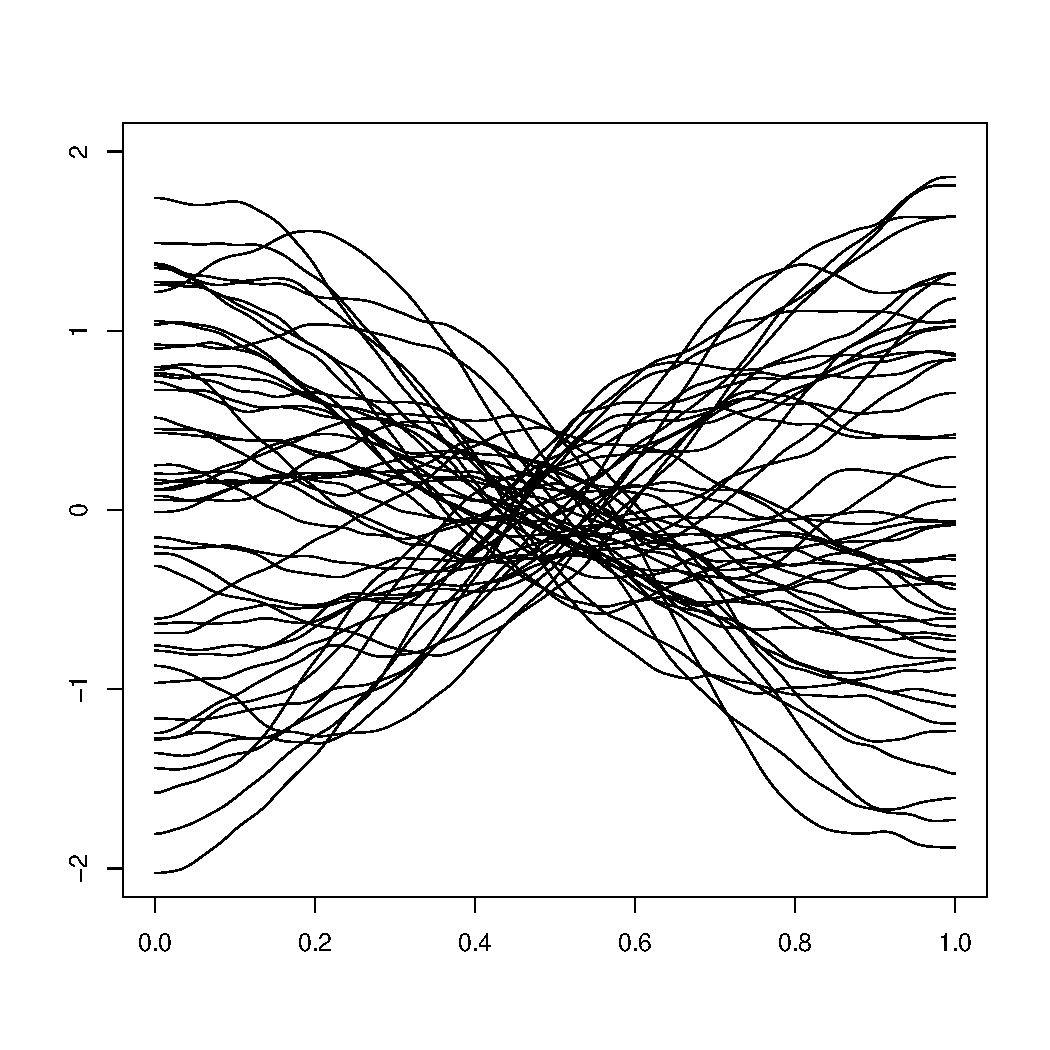
\includegraphics[width=\textwidth]{Plots/Images-nonparametric/cy-curves.pdf}
                \caption{}
                \label{}
        \end{subfigure}
         \begin{subfigure}[b]{0.34\textwidth}
                \centering
                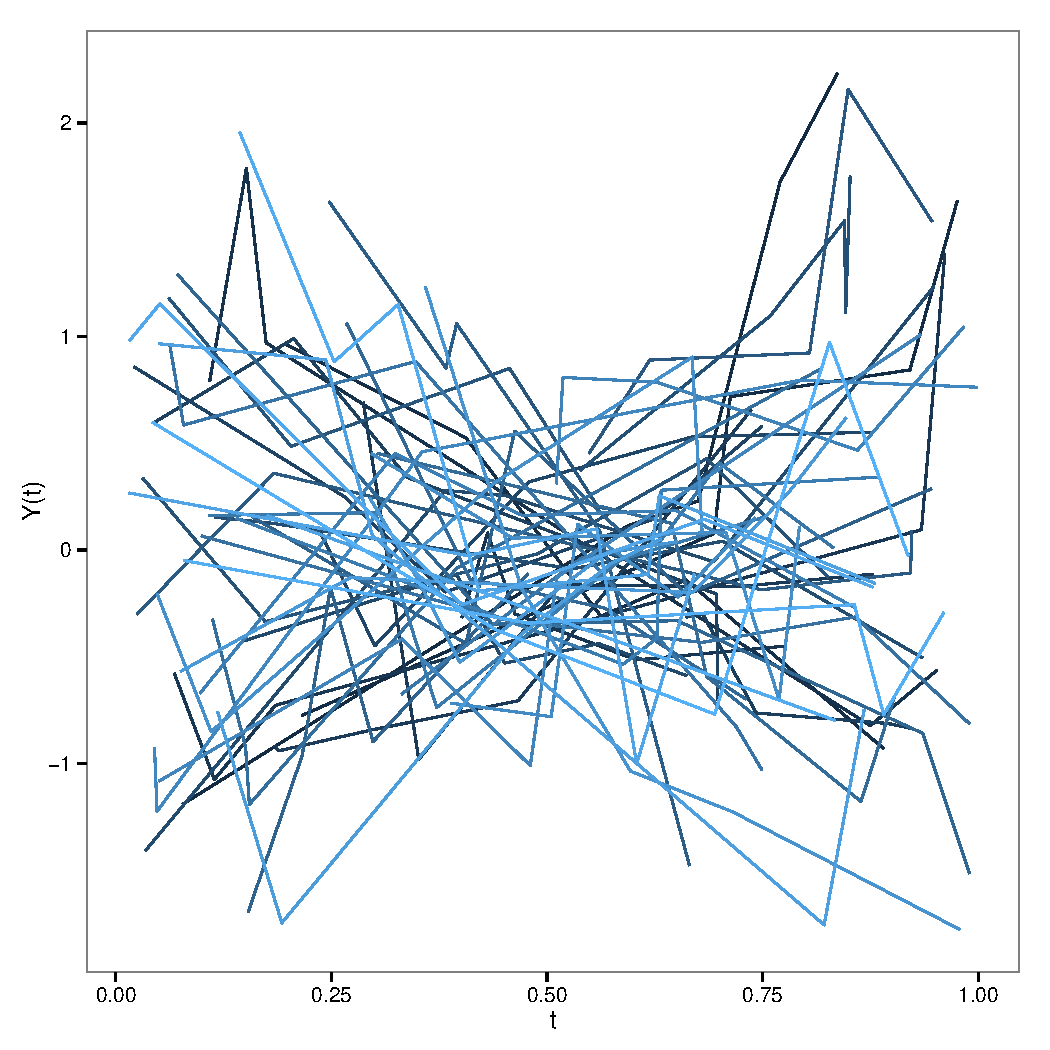
\includegraphics[width=\textwidth]{Plots/Images-nonparametric/cy-data-m5.pdf}
                \caption{}
                \label{}
        \end{subfigure}

        \begin{subfigure}[b]{0.34\textwidth}
                \centering
                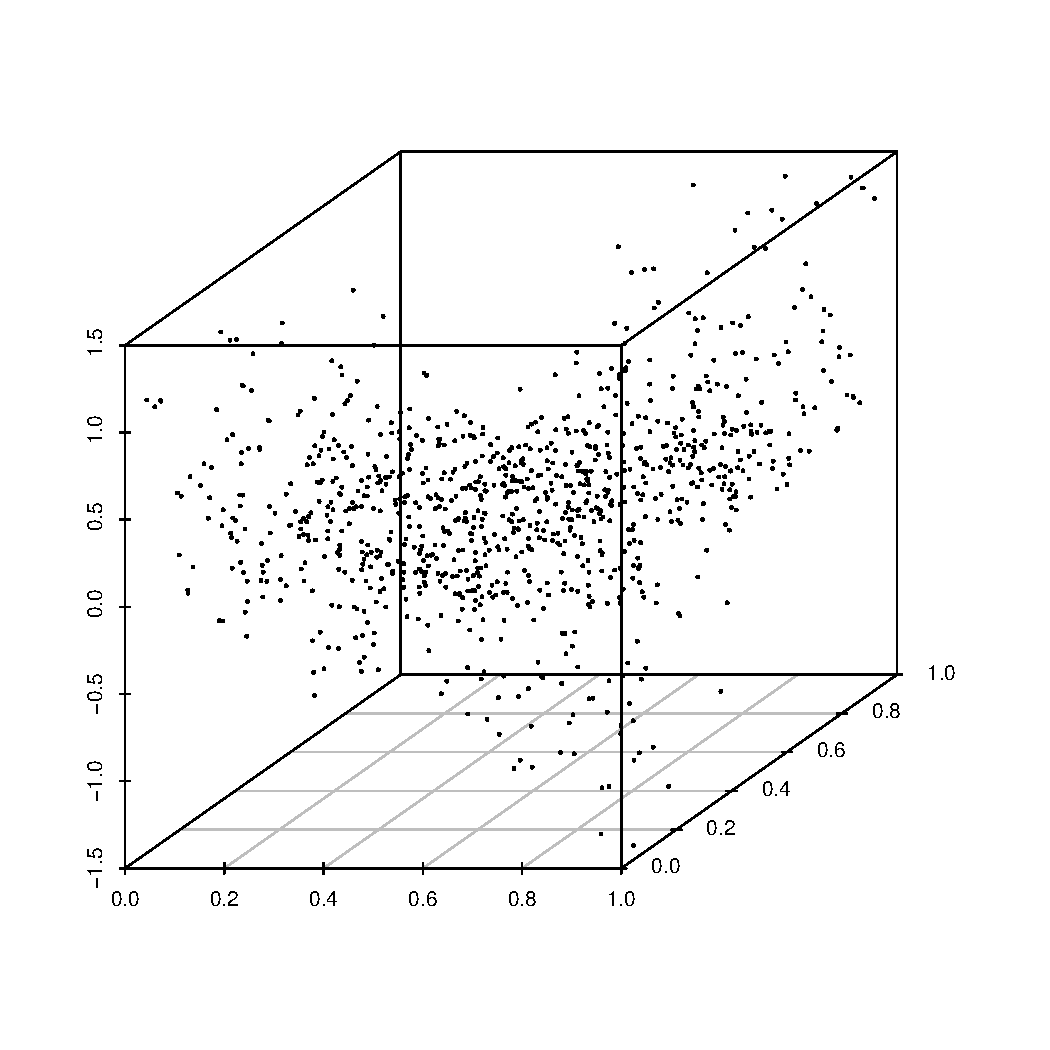
\includegraphics[width=\textwidth]{Plots/Images-nonparametric/cy-scatter3d-m5.pdf}
                \caption{}
                \label{}
        \end{subfigure}%
          \begin{subfigure}[b]{0.34\textwidth}
                \centering
                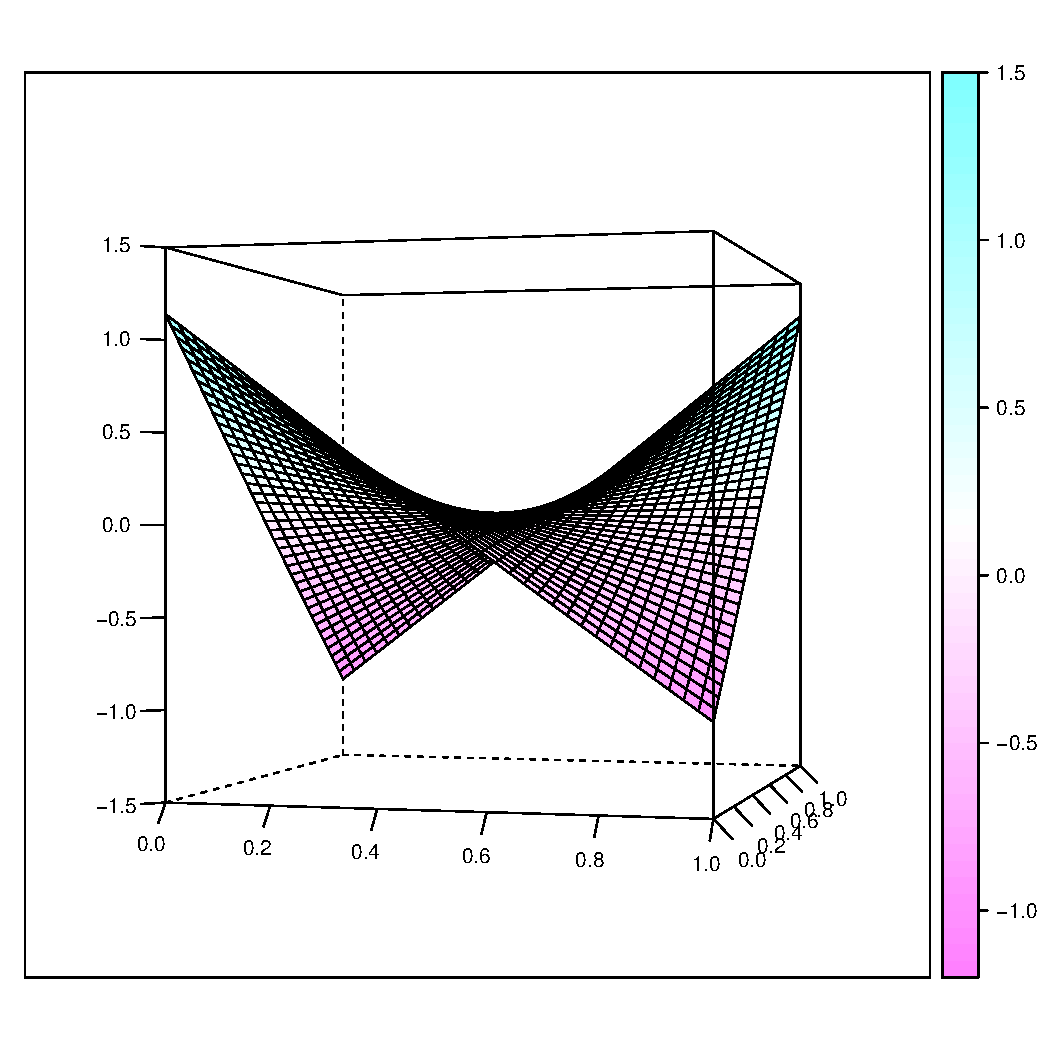
\includegraphics[width=\textwidth]{Plots/Images-nonparametric/cy-fit-wireframe-m5.pdf}
                \caption{}
                \label{}
        \end{subfigure}%
%        \caption{(a) 50 simulated curves from the process $X(t)$ in \eqref{eq:sim process} (b) data set of curves evaluated at five random locations with noise, $\sigma_0=0.392$ (c) Scatterplot of values based on the data used to estimate covariance surface (d) Estimated covariance function. }
%        \label{fig:sim curves}
 \end{figure}
}

\frame{
\begin{figure}
 	\centering   
        \begin{subfigure}[b]{.30\textwidth}
                \centering
                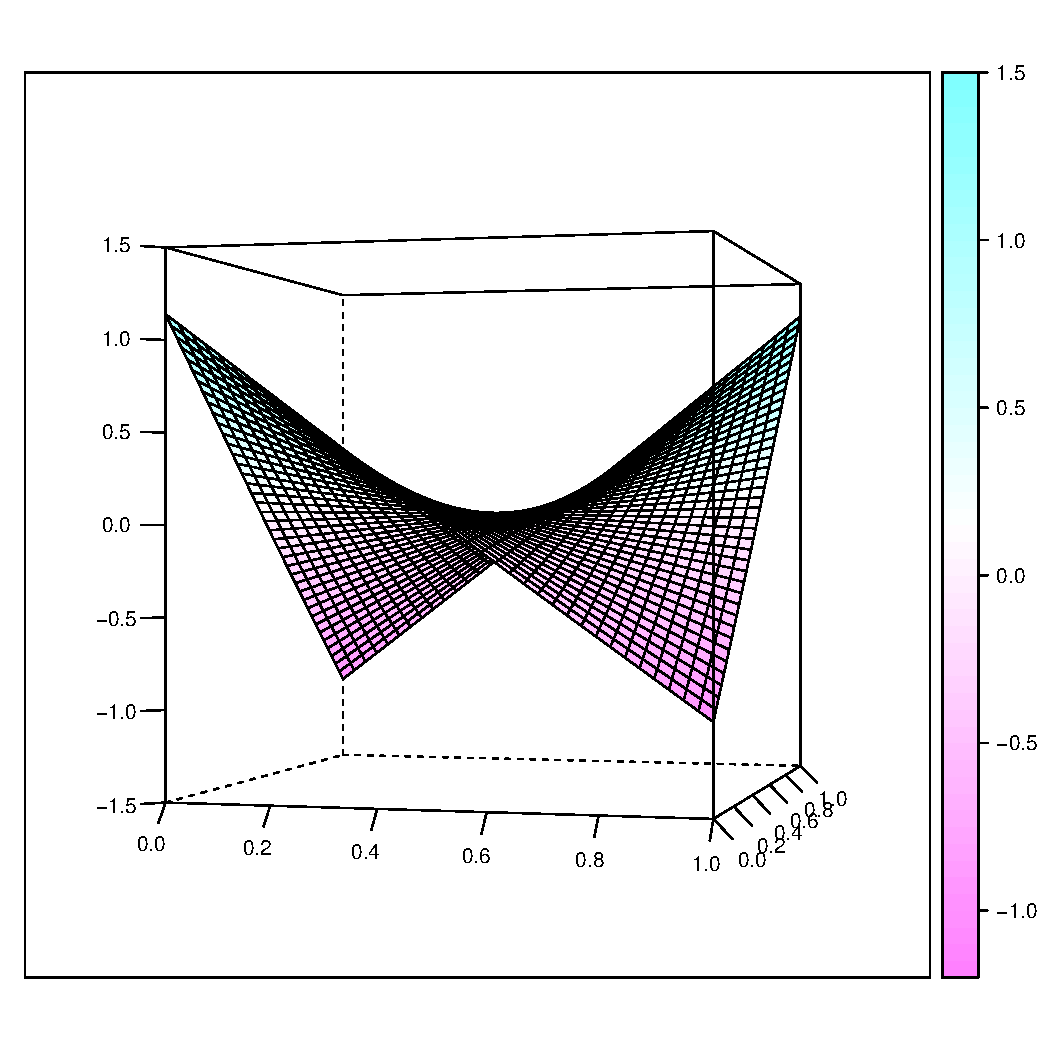
\includegraphics[width=\textwidth]{Plots/Images-nonparametric/cy-fit-wireframe-m5.pdf}
                \caption{m = 5}
                \label{}
        \end{subfigure}%
        \begin{subfigure}[b]{.30\textwidth}
                \centering
                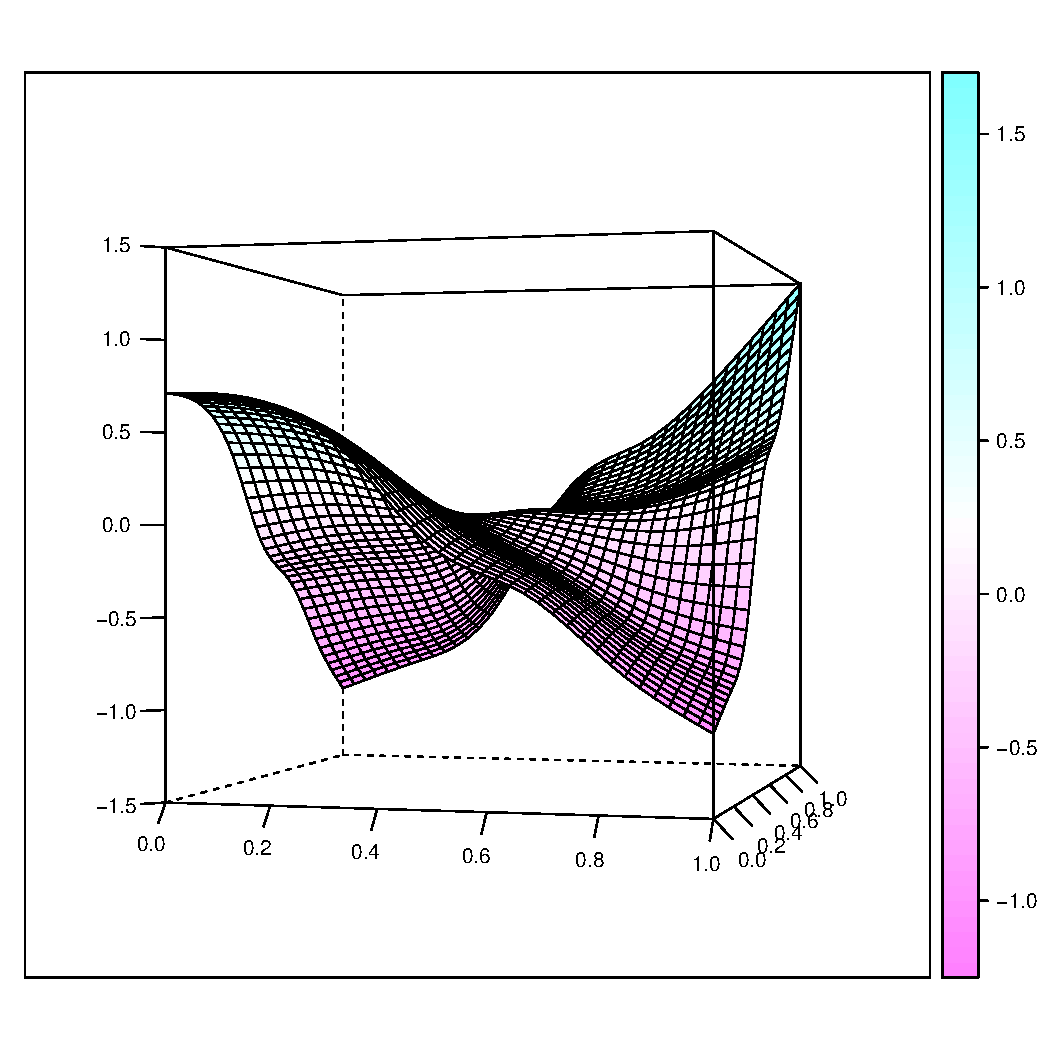
\includegraphics[width=\textwidth]{Plots/Images-nonparametric/cy-fit-wireframe-m10.pdf}
                \caption{m = 10}
                \label{}
        \end{subfigure}

        \begin{subfigure}[b]{.30\textwidth}
                \centering
                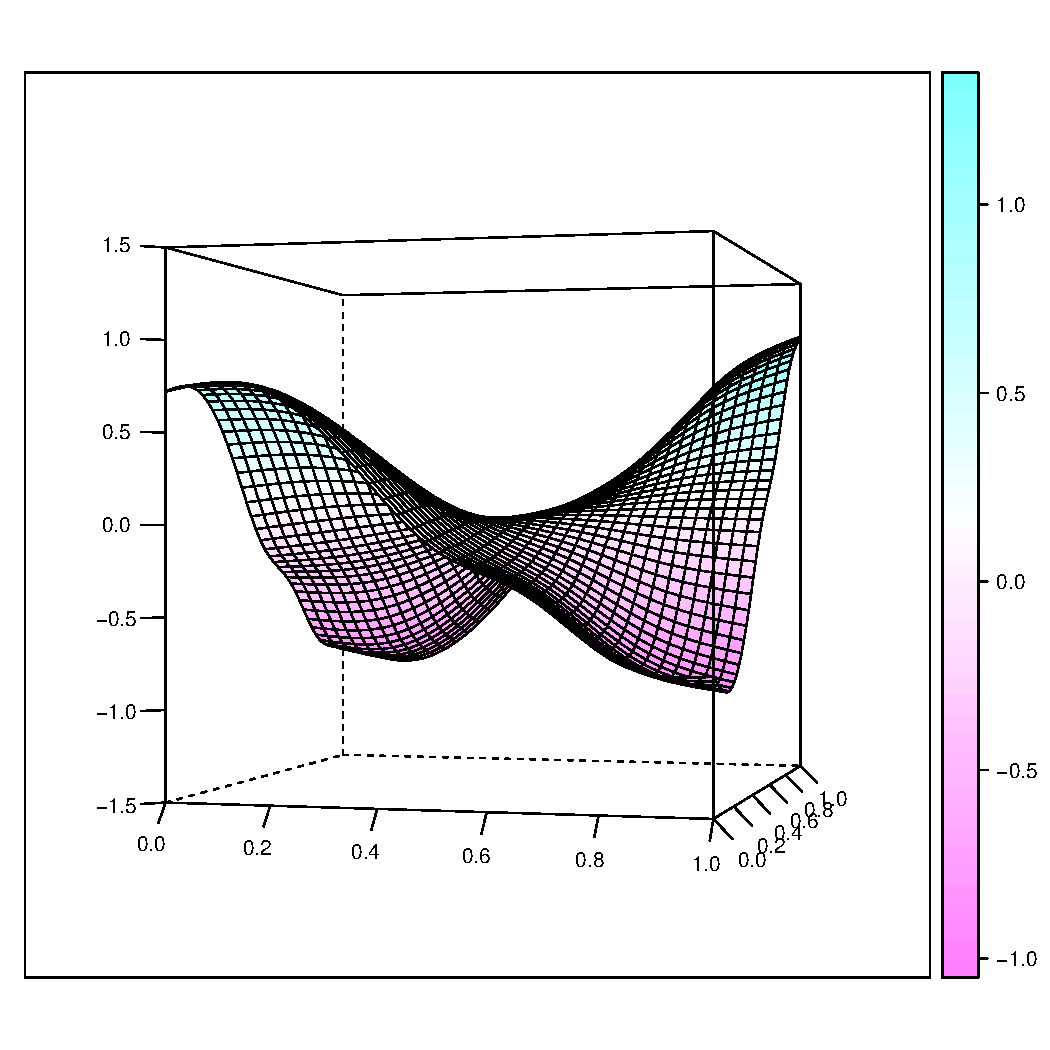
\includegraphics[width=\textwidth]{Plots/Images-nonparametric/cy-fit-wireframe-m40.pdf}
                \caption{m = 40}
                \label{}
        \end{subfigure}
                \begin{subfigure}[b]{.30\textwidth}
                \centering
                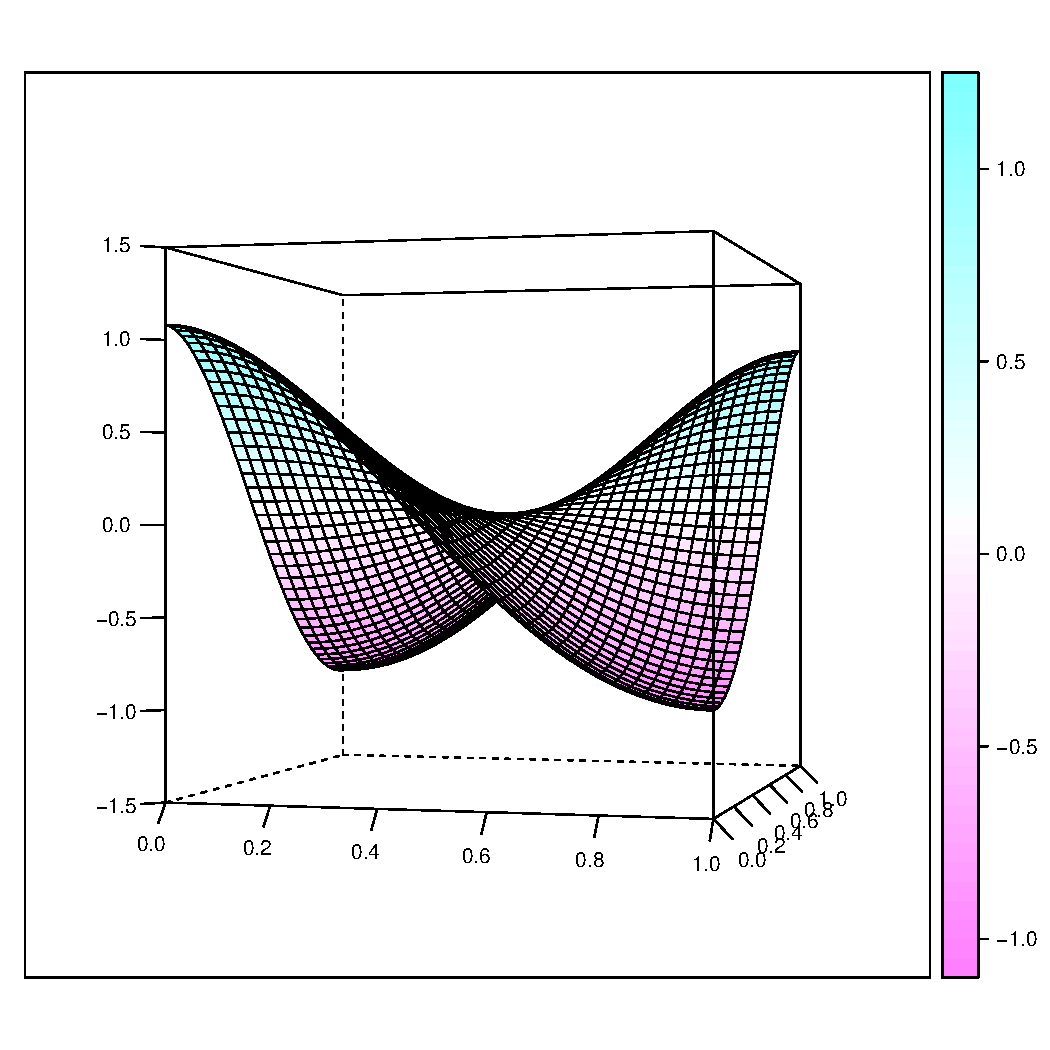
\includegraphics[width=\textwidth]{Plots/Images-nonparametric/cy-true-wireframe.pdf}
                \caption{truth}
                \label{}
        \end{subfigure}
\end{figure}
}


\begin{frame}
\frametitle{Functional Principal Components}
To the covariance $C(s,t)$ has the following representation 
\begin{equation*} 
 C(s,t) = \sum_{i=1}^{\infty}\lambda_i\psi_i(s)\psi_i(t),
\end{equation*}
\begin{itemize}
\item  $\{\psi_m(t)\}_{m=1,2,\ldots}$ are orthonormal (in $L_2$) eigenfunctions
\item  $\{\lambda_m \}_{m=1,2,\ldots}$ are nonnegative and nondecreasing eigenvalues. 
\item eigenfunctions satisfy $\int_a^bC(s,t)\psi_j(t)dt = \lambda_j\psi_j(t)$. 
\end{itemize}
Karhunen-Loeve theorem $\rightarrow$ $X(t)$ admits the representation
\begin{equation*}
X(t) =  \sum_{m=1}^{\infty}\alpha_m \psi_m(t), \mbox{ where  } \alpha_m = \int_a^b X(t) \psi_m(t)dt,
\end{equation*}
\begin{itemize}
\item $\{\alpha_m \}_{m=1,2,\ldots}$ are uncorrelated random variables
\item $E(\alpha_m)=0$ and Var($\alpha_m$) = $\lambda_m$, $\sum_m \lambda_m < \infty$. 
\end{itemize}
\end{frame}

\frame{

We seek functions $\hat{\psi}(s)$ that satisfy
\begin{equation*} \label{eq:eigenfuns}
\int \hat{C}(s,t)\hat{\psi}(t)dt=\theta\hat{\psi}(s).
\end{equation*}
\begin{itemize}
\item Idea: adapt methods developed for finite basis representations.
\item Let
\begin{equation}
\mathbf{g(\cdot)}=(1, k_1(\cdot),R_{1}(\cdot, t_1),R_{1}(\cdot, t_2),\dots, R_{1}(\cdot, t_K))'.
\label{eq:g}
\end{equation}
\item Need to represent $\hat{C}(s,t)= \mathbf{g}(s)'A\mathbf{g}(t)$ for some matrix $A$. See next slide...
\end{itemize}
}

\begin{frame}[shrink=10]
Using $\mathbf{g}$ in \eqref{eq:g} the covariance function estimator has the representation $\hat{C}(s,t)= \mathbf{g}(s)'A\mathbf{g}(t)$ where
\vspace{0.8cm}
\begin{center}
 $A = \left(\begin{array}{cc:cccc}
d_{00,00} & d_{01,00} & c_{1.} & c_{2.} & \dots & c_{K.}\\
d_{00,01} & d_{01,01} & \sum_j c_{1j}k_1(t_j) & \sum_j c_{2j}k_1(t_j) & \dots & \sum_j c_{Kj}k_1(t_j)\\
\hdashline
c_{.1}   & \sum_j c_{j1}k_1(t_j) & c_{11}   & c_{12}   & \dots & c_{1K}\\
c_{.2}   & \sum_j c_{j2}k_1(t_j) & c_{21}   & c_{22}   & \dots & c_{2K}\\
\vdots  & \vdots                            & \vdots    & \vdots & \ddots    & \vdots \\
c_{.K}   & \sum_j c_{jK}k_1(t_j) & c_{K1}   & c_{K2}   & \dots & c_{KK}
\end{array}\right)$
\end{center}
\end{frame}

\frame{
The following result states that the eigenfunctions can be expressed as a linear combination of the elements of $\mathbf{g}$.
\begin{lemma} \label{thm:eigenfunctions}
	The eigenfunctions of $\hat{C}(s,t)$ can be expressed as
	\begin{equation*}
		\hat{\psi}_k(\cdot) = b'_k\mathbf{g}(\cdot),	
	\end{equation*}
	where $Q$ is defined to be
\begin{equation*}
	Q_{ij} = \int_0^1\mathbf{g_i}(t)\mathbf{g}_j(t)dt,
\end{equation*}
	$b_k$ is the $k$-th column of $B=Q^{-1/2}U$ and $U$ is the eigenvectors of $Q^{1/2}AQ^{1/2}$, and 
\[
\mathbf{g(\cdot)}=(1, k_1(\cdot),R_{1}(\cdot, t_1),R_{1}(\cdot, t_2),\dots, R_{1}(\cdot, t_K))'.
\]
\end{lemma}
}


\frame{
\frametitle{Discussion}
\begin{itemize}
\item  Allows smoothing penalty to be more directly connected to the curves (i.e. the scientific process being observed). 
\item Simulation indicate the estimator performs well even with sparsely observed curves. 
\item Method is general and could easily be applied to a penalty based on arbitrary linear differential operators. 
\item We have also created an R package implementation, making it convenient to use empirical basis representation for functional data analyses. 
\end{itemize}
}


%%%%% PHENOLOGY %%%%%

\begin{frame}
\frametitle{Introduction}
\begin{itemize}
\item \emph{Phenology} is the study of annual life-cycles of terrestrial vegetation and how they are effected by climate change or other environmental variables. 

\item Understanding vegetation phenology and its spatio-temporal variation is required to reveal and predict ongoing changes in Earth system dynamics. \\[0.5cm]

\item \textbf{Goal}: Develop a flexible model for vegetation life-cycles.  A single life-cycle is determined by two variables: 
\begin{itemize} 
\item  
\item 
\end{itemize}
\end{itemize}
\end{frame}

\frame
{
\frametitle{Defining Vegetation Life-cycles}
\begin{figure}
   \begin{center}
   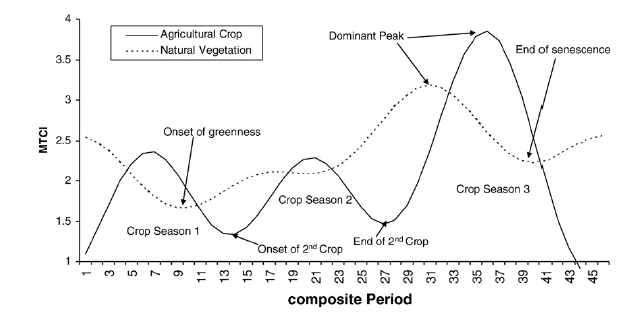
\includegraphics[width=\linewidth]{Plots/PhenoVars_Jegan.png} 
   %\caption{Diagram illustrating typical phenology patterns for agricultural land and natural vegetation. }
\end{center}
\end{figure}
}

\frame
{
\frametitle{Data processing and analysis flow chart }
\begin{figure} %  figure placement: here, top, bottom, or page
   \begin{center}
   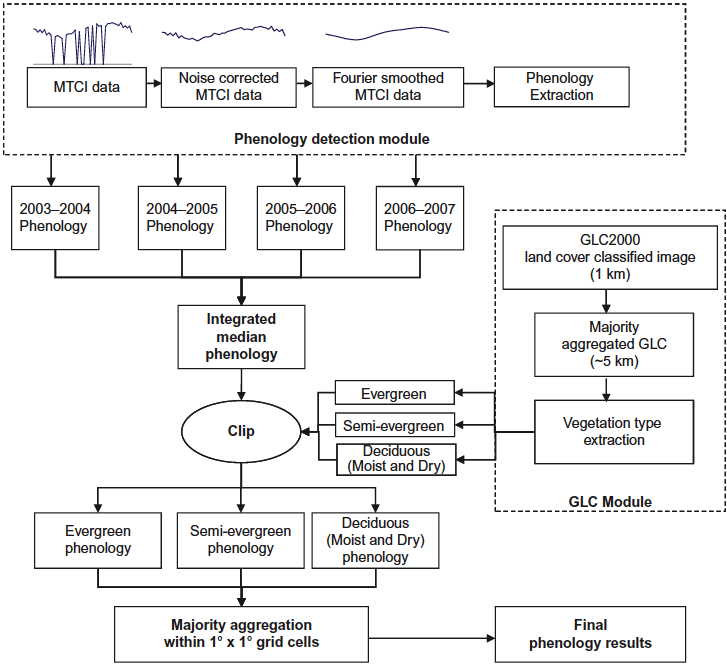
\includegraphics[width=0.7\linewidth]{Plots/PhenoScheme.png} 
%   \caption{example caption}
   %\label{fig:example}
   \end{center}
\end{figure}
}

\frame
{
\frametitle{Data processing and analysis flow chart }
\begin{figure} %  figure placement: here, top, bottom, or page
   \begin{center}
   \includegraphics[width=\linewidth]{Plots/pheno-diagram.png} 
%   \caption{example caption}
   %\label{fig:example}
   \end{center}
\end{figure}
}

\begin{frame}[t]{Study region in southern India: Satellite image from May 2000}
	\includegraphics[width=0.95\linewidth]{Images-phenology-fda/Satellite/India_zoom.png} 
\end{frame}
%--- Next Frame ---%

\begin{frame}[t]{GLC2000 Global Land Cover classification \\@ 4.6 km by 4.6 km spatial resolution}
	\begin{figure} 
		%\includegraphics[width=0.35\linewidth]{Images-phenology-fda/Satellite/India-5-12-2000.png}   
		\includegraphics[width=\linewidth]{Images-phenology-fda/land_cover.pdf} 
		%\caption{Land cover classification at 4.6~km spatial resolution derived from GLC2000 land cover database.} \label{fig:land cover} 
	\end{figure}
\end{frame}
%--- Next Frame ---%

\begin{frame}[t]{Mean MTCI by landcover for 2003 - 2007}
	\begin{figure}    
		\includegraphics[width=\linewidth]{Images-phenology-fda/mean_by_LC_facet_year.pdf} 
		%\caption{Land cover classification at 4.6~km spatial resolution derived from GLC2000 land cover database.}
	\end{figure}
\end{frame}
%--- Next Frame ---%

\begin{frame}[t]{Agriculture and Natural Vegetation Land Cover}
	\begin{minipage}{0.48\textwidth}
		\begin{figure}
		\includegraphics[width = \textwidth]{Images-phenology-fda/Plots/proportion_agriculture.pdf}
	%	\caption{Proportion of agricultural landcover using GLC2000 database}
		\end{figure}
	\end{minipage}
	\begin{minipage}{0.48\textwidth}
		\begin{figure}
		\includegraphics[width = \textwidth]{Images-phenology-fda/Plots/landcover_ag_veg.pdf}
	%		\caption{Black pionts are homogeneous agriculture locations}
		\end{figure}
	\end{minipage}
	
	\begin{minipage}{0.48\textwidth}
	\begin{itemize}
		\item Proportion Agriculture
		\item based on GLC2000 database
	\end{itemize}
	\end{minipage}
	\begin{minipage}{0.48\textwidth}
	\begin{itemize}
		\item black points indicate homogeneous agriculture cells
		\item homogeneous agriculture = 100\% agriculture landcover
	\end{itemize}
	\end{minipage}
\end{frame}
%--- Next Frame ---%

\begin{frame}[t]{Modeling Approach}
	 Our general approach consists of the following steps:
	\begin{enumerate}
		\item Label each cell as either vegetation, agriculture, or other. 
		\item Construct a set of empirical basis functions derived from land that is primarily agricultural. 
		\item Project all of the data onto this basis, reducing the information for each curve to a low dimensional vector of coefficients.
		\item Construct a classifier for the coefficient vectors by using a training set corresponding to the homogeneous agriculture locations and an equal number of homogeneous vegetation locations.  
	\end{enumerate}
\end{frame}

\begin{frame}[t]{title}
	To produce smooth estimates of the trajectories $X_i(t)$, project the observations $Y_i(t_j), j = 1, \dots, 46$ onto the finite dimensional functional basis $\{\hat{\psi}_k(t), k = 1, \dots, q\}$, where $q$ is chosen such that at least $90\%$ of the variation is explained. The fitted trajectories admit the following representation
	\begin{equation}
		\widehat{X_i(t)} = \sum_{k=1}^q\alpha_{k,i} \hat{\psi}_k(t) = \boldsymbol{\alpha_i'}\boldsymbol{\psi}.
		\label{phen:coef}
	\end{equation}
	In this representation the randomness associated with each random trajectory $X(t)$ is captured in the coefficient vector $\boldsymbol{\alpha}$. This allows one to take advantage the vast methods available for multivariate data.
\end{frame}
%--- Next Frame ---%

%--- Next Frame ---%

\begin{frame}[t]{Classification Model}
	\textbf{Linear Discriminant Analysis (LDA)} % (fold)
	
	Let C be a random variable taking values in $\mathcal{C} = \{ \text{Agriculture}, \text{Vegetation}\} = \{\text{A}, \text{V}\}$. 
	\begin{equation*}
		\hat{\text{C}}(\boldsymbol{\alpha}) = 
		\begin{cases}
				\text{A} \hfill & \text{ if } \text{Pr}(\text{C = A }| \boldsymbol{\alpha})> \text{Pr}(\text{C = V }| \boldsymbol{\alpha})\\
				\text{V} \hfill & \text{ otherwise}
		\end{cases}
	\end{equation*}  
	Computation of the posterior probabilities follows from modeling the class-conditional densities $f_k(\boldsymbol\alpha)$ as multivariate Gaussian distributions
	\begin{equation*}
		f_k(\boldsymbol\alpha) = \frac{1}{(2\pi)^{p/2}}e^{-\frac{1}{2}(\boldsymbol\alpha - \boldsymbol\mu_k)^T\Sigma^{-1}(\boldsymbol\alpha - \boldsymbol\mu_k)}
	\end{equation*}
	LDA assumes common covariance matrix between classes. 
	\begin{equation*}
		\text{Pr}(\text{C} = \text{A } | \boldsymbol\alpha) = \frac{f_{A}(\boldsymbol\alpha)\pi_{A}}{f_{A}(\boldsymbol\alpha)\pi_{A}+f_{V}(\boldsymbol\alpha)\pi_{V}}
	\end{equation*}
	where $\pi_{A}$ and $\pi_{V}$ are the prior probabilities class membership.
\end{frame}
%--- Next Frame ---%

\begin{frame}{Classification Results}
	\begin{minipage}{0.45\textwidth}
		\begin{figure}
		\includegraphics[width = \textwidth]{Images-phenology-fda/Plots/prob_ag.pdf}
		\caption{Posterior probability of `Agriculture'}
		\end{figure}
	\end{minipage}
	\begin{minipage}{0.45\textwidth}
		\begin{figure}
		\includegraphics[width = \textwidth]{Images-phenology-fda/Plots/misclassified_vegetation.pdf}
		\caption{RED = disagreement with GLC2000}
		\end{figure}
	\end{minipage}
\end{frame}
%--- Next Frame ---%


\begin{frame}[t]{Classification Results: 2007}
	\begin{minipage}{.4\textwidth}
	\includegraphics[width = .8\textwidth]{Images-phenology-fda/Plots/classification-2007.png}\\
	\includegraphics[width = .8\textwidth]{Images-phenology-fda/posterior_probs_2007.png}
	\end{minipage}
	\begin{minipage}{.5\textwidth}
	 \begin{itemize}
	 	\item Classification disagreement in the year 2007
		\item Red areas are classified as agricultural land 
	 \end{itemize}
	\end{minipage}
\end{frame}
%--- Next Frame ---%

\begin{frame}[t]{Classification Results: 2007}
	\begin{figure}
		[htbp] \centering 
		\includegraphics[width=0.5\linewidth]{Images-phenology-fda/Plots/landcover_overlay_background.png} \\[0.1cm]
		\includegraphics[width=0.5\linewidth]{Images-phenology-fda/Plots/landcover_overlay.png} \\
		\caption{Satellite image of northwestern part of the study region in southern India in 2014 (top). Areas in the year 2007 designated as agricultural by the LDA classifier, but labeled as vegetation by the GLC2000 database are shown in red (bottom).} 
	\end{figure}
	
\end{frame}
%--- Next Frame ---%

\begin{frame}[t]{Summary \& Conclusions}
	\begin{itemize}
		\item FPC representation allows multivariate methods to be utilized in FDA
		\item Described a fully nonparemetric estimator for computing FPCs
	\end{itemize}
	
\end{frame}
%--- Next Frame ---%


%=========================================================
% Spatial Functional Data: Estimation and Prediction with kriging
%=========================================================

\frame{
\begin{center}
ESTIMATION AND KRIGING FOR SPATIALLY INDEXED FUNCTIONAL DATA
\end{center}
}
\frame
{
\begin{figure}
\begin{center}
\includegraphics[width=3in]{Plots/canadian-weather.pdf}
\caption{ Mean monthly temperatures for Canadian weather stations.}
\end{center}
\end{figure}
}


\frame
{
\frametitle{Geostatics for scalar valued random fields}
\[
	 \left\{ \boldsymbol\chi_s: s \in D  \subseteq \Real^2\right\} 
\] 
data: $\left\{ \chi_{s_1}, \chi_{s_2}, \dots, \chi_{s_n} \right\} \hspace{0.2cm} i = 1, \dots, n$

Kriging predictor (Best linear unbiased predictor):

\[
\widehat{\chi_{s_0}} = \sum_{i=1}^n \lambda_i \chi_{s_i}
\]
Unbiased constraint: 
\[
\sum_{i=1}^n \lambda_i = 1
\]
Weights $\lambda_i$ are determined by the variogram
\[
\gamma(h) = \frac{1}{2}Var(\chi_{s+h} -\chi_s)
\]
}

\frame
{
  \textbf{Spatial functional process:}\\
	\[
	 \left\{ \boldsymbol\chi_s(\cdot): s \in D  \subseteq \Real^2\right\} 
	 \] 
	 
	$\boldsymbol\chi_s(\cdot)$ second order stochastic process on a compact set $\mathcal{T} \subset \Real$\\[0.2cm]
	
	\textbf{What we actually observe}:\\[0.2cm]
	
	$y_{i,j} = \chi_{s_i}(t_j) + \epsilon_{i,j} \hspace{1cm} i = 1,\dots, n; \hspace{0.2cm} j = 1,\dots, m_i$\\[0.3cm]
	
	$n =$ number of curves\\
	$m_i=$ number of observations on curve $i$
}

\frame
{
First attempt at functional geostatistics: Goulard and Volts (1993)
\begin{itemize}
\item{\textbf{Method 1}} functional version of the variogram
\item{\textbf{Method 2}} fitting curves, cokriging the coefficients\\[0.2cm]
\end{itemize}
Giraldo, Delicado, and Mateu (2011) extend \textbf{Method 1}
\begin{itemize}
\item assume $\chi_s(t)$ take values in $L_2(\T)$
\item estimate curves non-parametrically using B-splines
\item Functional Variogram \[ \gamma(h) = \frac{1}{2}E\left[ \int_{\T}(\chi_t(s_i) - \chi_t(s_j))^2 dt \right] , h = \norm{s_i - s_j}\]
\item Predictor \[
\widehat{\chi_{s_0}(t)} = \sum_{i=1}^n \lambda_i \chi_{s_i}(t)
\]
\end{itemize}
%Nerini, Monestiez, Mant\'e (2009) extend \textbf{Method 2}
%\begin{itemize}
%\item assume $\chi_s(t)$ take values in a Reproducing Kernel Hilbert Space
%\item project sample curves into an orthogonal basis (Legendre polynomials)
%\end{itemize}
}



\frame
{
\frametitle{Our Approach extends method 2}
\begin{itemize}
\item We assume $\boldsymbol\chi(s; \cdot)$  takes values in a RKHS $\H$. \\[0.2cm]
\item $\chi(s;t)$ admit the following representation 
\begin{equation}
 	\chi(s;t) = \mu(t) + \epsilon(s;t),
\end{equation}
where $\mu(t)$ represents large-scale structure which does not depend on spatial location and $\epsilon(s;t)$ is a mean zero spatially correlated random effect. 
 \item $\epsilon(s;t)$ can be represented by the Karhunen-Loeve expansion $\epsilon(s;t) = \sum_{k=1}^{\infty} \alpha_k(s)\psi_k(t)$. 
 \item For each integer $k$, $\alpha_k(s) = \inner{\epsilon(s;t)}{ \psi_k(t)}$ is assumed to be a second-order stationary isotropic random field. 
 \item Spatial random fields connected to different eigenfunctions are assumed to be uncorrelated, that is 
\begin{equation}
	\text{Cov}(\alpha_j(s), \alpha_l(s')) = 0 \hspace{1cm} \text{for } j \neq l.
	\label{eq:nocrosscor}
\end{equation} 
\end{itemize}
}

\begin{frame}
The covariance between curves at locations $s_j$ and $s_l$ are given by 
\begin{align}
	\text{Cov}(\chi(s_j,t), \chi(s_l, t')) &= \sum_{k=1}^{\infty}\text{Cov}(\alpha_k(s_j), \alpha_k(s_l))\psi_k(t)\psi_k(t')\\
	&= \sum_{k=1}^{\infty}h_k(\norm{s_j-s_l})\psi_k(t)\psi_k(t'). 
	\label{eq:cov}
\end{align}

In practice we work with the truncated expansion $\epsilon(s;t) = \sum_{k=1}^{q} \alpha_k(s)\psi_k(t)$, where $q$ is chosen to preserve most of the (interesting/low frequency) variation. Estimation of the eigenfunctions is done using a method described earlier.
\end{frame}


\frame
{
Steps for prediction at unobserved location $s_0$:
\begin{enumerate}
\item project sample curves into eigenfunctions: $\hat{\psi}^{(1)}, \hat{\psi}^{(2)}, \dots, \hat{\psi}^{(q)}$ 
\item compute kriging estimates of the coefficients: $\hat{\alpha}_{s_0}^{(1)}, \hat{\alpha}_{s_0}^{(2)}, \cdots, \hat{\alpha}_{s_0}^{(q)}$ 
\item $\widehat{\chi_{s_0}(t)}_{ok} = \sum_{k=1}^{q} \hat{\alpha}_{s_0}^{(k)}\hat{\psi}^{(k)}(t)$
\end{enumerate}

}


\begin{frame}
\frametitle{Adjustments to the covariance function estimation which account for spatial dependence}

Let $\mathbf{b}^{(i)} = [(y_{ij}-\mu(t_{ij}))(y_{ij'}-\mu(t_{ij'}))]_{1\leq j\neq j'\leq m}$, $i=1, \dots, n$. Let
\[
\mathbf{b} = (\mathbf{b}^{(1)T}, \mathbf{b}^{(2)T}, \dots, \mathbf{b}^{(n)T}   )^T,
\]
 The elements of $\mathbf{b}$ have non-trivial covariances due to spatial correlation among curves. However, we show that the elements of Cov$(\mathbf{b})$ can be compute using only covariances of the form \eqref{eq:cov}. Let
\[
\mathbf{W}= \text{Cov}(\mathbf{b}), 
\]

then elements of $\mathbf{W}$ can be computed as follows,
\begin{align} 
	&\text{Cov}(\epsilon(s_i; t_{j}) \epsilon(s_i;t_{j'}), \epsilon(s_{i'}; t_{l}) \epsilon(s_{i'};t_{l'}) ) \nonumber\\
	&= 
	  \text{Cov}(\epsilon(s_i; t_{j}), \epsilon(s_{i'}; t_{l}))\text{Cov}( \epsilon(s_i;t_{j'}), \epsilon(s_{i'};t_{l'})  ) \nonumber \\
	&+
		 \text{Cov}(\epsilon(s_i; t_{j}),  \epsilon(s_{i'};t_{l'}) )\text{Cov}(\epsilon(s_i;t_{j'}), \epsilon(s_{i'}; t_{l})) \label{eq:cov of products}
\end{align}
The right hand side of \eqref{eq:cov of products} holds under the assumption of Gaussian distributions (see Bohrnstedt). 
\end{frame}

\begin{frame}
We propose the following estimator
\[
\widehat{C}_{\lambda}=\stackrel[C \in \H\otimes \H]{}{\text{ argmin}} \left\{ l_{n}(C)+\lambda\left\Vert C\right\Vert _{\breve{\H}}^{2} \right\},
\]
 where

\begin{equation}
l_{n}(C)= (\mathbf{b} - \mathbf{C})^T\mathbf{W}^{-1}(\mathbf{b} - \mathbf{C})
\label{eq:weighted loss function}
\end{equation}
and 
\[
\mathbf{C} = [C(t_{i,j}, t_{i'j'})]
\]
\end{frame}
%=====================================


\begin{frame}[t]{}
	\begin{figure}[h]
		\begin{center}
			\includegraphics[width=0.7\textwidth]{Images-ordinary-kriging/Plots/grid.pdf} 
		\end{center}
		\caption{Locations of curves used for the simulation.} \label{fig:grid3} 
	\end{figure}
\end{frame}
%--- Next Frame ---%

\begin{frame}[t]{}
	\begin{figure}[h]
		\begin{center}
			\includegraphics[width=0.7\textwidth]{Images-ordinary-kriging/Plots/exp_corr_funs.pdf} 
		\end{center}
		\caption{Exponential covariance functions used in the simulation.} \label{fig:exp_corr_funs} 
	\end{figure}
\end{frame}
%--- Next Frame ---%

\begin{frame}[t]{}
	\begin{figure}[h]
		\begin{center}
			\includegraphics[width=\textwidth]{Images-ordinary-kriging/Plots/MSE_trends.pdf} 
		\end{center}
		\caption{The x-axis shows the value of the scale parameter, $p$, in the weight function. Large values of $p$ correspond to smaller weights for curves in high point intensity areas. The y-axis shows the average integrated square error for the covariance estimator. The error bars show +/- two standard errors.} \label{fig:MSE_trends} 
	\end{figure}
\end{frame}
%--- Next Frame ---%

\begin{frame}[t]{}
\begin{table}
	\begin{center}
	\caption{Correlation values corresponding to locations on the simulation grid (Figure~\ref{fig:grid3}) for each level of spatial dependence. The table shows the largest correlation among the subset of dense locations, and the largest correlation among the subset of sparse locations. Spatial dependence is represented by the value of the range parameter $r$ in the exponential covariance function in \eqref{eq:exp cov}.}
\begin{tabular}{|c|c|c|}
	\hline
	range $r$ & dense locations & sparse locations \\
	\hline
	0.1 & 0.7 & 0.1 \\
	0.2 & 0.8 & 0.4 \\
	0.3 & 0.9 & 0.5 \\
	\hline
\end{tabular}
\label{tab:corr values}
\end{center}
\end{table}
\end{frame}
%--- Next Frame ---%

\begin{frame}[t]{}
	\begin{itemize}
		%\item IND: This method uses the overall mean as the prediction for each location.
		\item CFPC: Cokriging functional principal components. This is the (un-weighted) estimator developed in this paper.
		\item CFPCw: same, but using the weighted covariance estimator with $p=0.5$.
		\item OKFD: Ordinary kriging of functional data (Giraldo 2011)
	\end{itemize}
\end{frame}
%--- Next Frame ---%

\begin{frame}[t]{}
	\begin{minipage}{0.4\textwidth}
		\begin{figure}
			\begin{center}
				\includegraphics[width=\textwidth]{Images-ordinary-kriging/Plots/pred_locations.pdf} 
			\end{center}
			\caption{Spatial locations. Red = unobserved.} 
		\end{figure}
	\end{minipage}
	\begin{minipage}{0.5\textwidth}
		\begin{figure}
			\begin{center}
				\includegraphics[width=\textwidth]{Images-ordinary-kriging/Plots/pred_curves_exp.pdf} 
			\end{center}
			\caption{Predicted curves\\ Black = Truth\\ Params: $r = 0.2$, m = 20, $\sigma_0 = 0.3$.  } 
		\end{figure}
	\end{minipage}
\end{frame}
%--- Next Frame ---%

\begin{frame}[t]{}
	\begin{figure}
		\begin{center}
			\includegraphics[width=\textwidth]{Images-ordinary-kriging/Plots/kriging_boxplots_all.pdf} 
		\end{center}
		\caption{Boxplots showing distribution of the average prediction error, $\norm{\hat{X}(t) - X(t)}^2_{L_2}$, across the 12 unobserved locations for 100 simulated data sets. The plot label `sigma' refers to the observation error standard deviation $\sigma_0$. } 
	\end{figure}
\end{frame}
%--- Next Frame ---%

\begin{frame}[t]{Conclusions}
	\begin{itemize}
		\item Downweighting clustered curves improves covariance function estimation
		\item Spatial prediction is slightly improved
		\item Prediction performance is matches that of standard functional kriging
		\item Better suited for sparse functional data
		\item If observations on curves are both sparse and not from common distribution, then pooling data across curves may be the only suitable approach. 
	\end{itemize}
	
\end{frame}
%--- Next Frame ---%


%===========================================
% Bibliography
%===========================================
%\begin{frame}{Bibliography}
%\bibliographystyle{asa}
%\bibliography{bib-dissertationnew.bib,bib-books.bib}
%\end{frame}


\end{document}









